\documentclass [aspectratio=169]{beamer}
\beamertemplatenavigationsymbolsempty
\usetheme{Boadilla}
\usepackage{textpos} % package for the positioning
\usepackage[]{graphicx}
\usepackage{graphicx}
\usepackage{float}
\usepackage{hyperref}
\usepackage{caption}
\usepackage{subcaption}
\usepackage{algorithm,algpseudocode}
\usepackage[export]{adjustbox}
\usepackage{tikz}
\usetikzlibrary{positioning}

\usepackage[square,numbers]{natbib}
\usepackage[byname]{smartref}
\usetikzlibrary{positioning}
\usetikzlibrary{arrows, shapes, decorations, automata, backgrounds, fit, petri, calc}

\newcommand*{\logofont}{\fontfamily{phv}\selectfont}

\definecolor{uwopurple}{RGB}{79,38,131} % official purple color for uwo

\title[]{\vspace{60pt} \\
SleepGCN-Transformer: A Hybrid Graph Convolutional and Transformer Network for Sleep Stage Classification} % Change the lecture topic right here!
%\subtitle{n}
\author[]{Tanmay Rathod }
\large \institute[]{Under the guidance: Dr. Santosh Kumar Satapathy\\ [5pt]
Assistant Professor, Department of ICT, PDPU Gandhinagar}

\date{May 21, 2025}

% Math notations
\newtheorem{thm}{Theorem}[section]
\newtheorem{lem}[thm]{Lemma}

\newtheorem{defn}[thm]{Definition}
\newtheorem{eg}[thm]{Example}
\newtheorem{ex}[thm]{Exercise}
\newtheorem{conj}[thm]{Conjecture}
\newtheorem{cor}[thm]{Corollary}
\newtheorem{claim}[thm]{Claim}
\newtheorem{rmk}[thm]{Remark}

\newcommand{\ie}{\emph{i.e.} }
\newcommand{\cf}{\emph{cf.} }
\newcommand{\into}{\hookrightarrow}
\newcommand{\dirac}{\slashed{\partial}}
\newcommand{\R}{\mathbb{R}}
\newcommand{\C}{\mathbb{C}}
\newcommand{\Z}{\mathbb{Z}}
\newcommand{\N}{\mathbb{N}}
\newcommand{\Q}{\mathbb{Q}}
\newcommand{\LieT}{\mathfrak{t}}
\newcommand{\T}{\mathbb{T}}
\newcommand{\A}{\mathds{A}}
\newcommand{\E}{\mathbb{E}}
\newcommand{\Prob}{\mathbb{P}}
\newcommand{\Var}{\text{Var}}
\newcommand\equalhat{%
\let\savearraystretch\arraystretch
\renewcommand\arraystretch{0.3}
\begin{array}{c}
\stretchto{
    \scalerel*[\widthof{=}]{\wedge}
    {\rule{1ex}{3ex}}%
}{0.5ex}\\ 
=%
\end{array}
\let\arraystretch\savearraystretch
}

% set color
\setbeamercolor{title in head/foot}{bg=white}
\setbeamercolor{author in head/foot}{bg=white}
\setbeamercolor{date in head/foot}{fg=uwopurple}
\setbeamercolor{date in head/foot}{bg=white}
\setbeamercolor{title}{fg=uwopurple}
\setbeamerfont{title}{series=\bfseries}
\setbeamercolor{frametitle}{fg=uwopurple}
\setbeamerfont{frametitle}{series=\bfseries}
\setbeamercolor{block title}{bg=uwopurple!30,fg=black}
\setbeamercolor{item}{fg=uwopurple}
\setbeamercolor{caption name}{fg=uwopurple!70!}









 

 
\begin{document}

{
\setbeamertemplate{logo}{}
\begin{frame}
    \titlepage
    \begin{textblock*}{4cm}(0.5cm,-7.3cm)
        
\includegraphics[width=4cm]{figures/pdpu logo-.png}
    \end{textblock*}
    \begin{textblock*}{8cm}(5.0cm,-7.0cm)
        \huge \color{uwopurple}{$\Bigr\rvert$ \hspace{0.15cm} \textbf{Project Seminar}} % Change the lecture # right here! 
    \end{textblock*}
\end{frame}
}




\begin{frame}{SleepGCN-Transformer}

    \begin{block}{}
        \begin{itemize}
        	\item \textbf{1. Problem Statement}
            \item \textbf{2. Abstract}
            \item \textbf{3. Introduction}
            \item \textbf{4. Methodology}
            \item \textbf{5. Results}
            \item \textbf{6. Future Plan \& Conclusion}
        \end{itemize}
    \end{block}
\end{frame}

    \begin{frame}{Problem Statement}
	\begin{block}{\centering \textbf{Problem Statement}}
		\centering
		\textbf{Automated Sleep Stage Classification Using EEG Signals: A Machine Learning Approach with Feature-Based Modeling and K-Fold Validation}
	\end{block}
\end{frame}

     \begin{frame}{Abstract}
    \textbf{Dataset:} \textbf{SleepEDF} dataset. \\[5pt]

    \textbf{Preprocessing:} Using 4 selected channels:  
    \begin{itemize}
        \item EEG Fpz-Cz
        \item EEG Pz-Oz
        \item EMG submental
        \item EOG horizontal
    \end{itemize}

    \textbf{Methodology:}  
    \begin{itemize}
        \item \textbf{Graph Convolutional Neural Network (GCN)} 
        \item \textbf{Transformer Encoder}  
    \end{itemize}

    \textbf{Results:}  
    \begin{itemize}
        \item \textbf{Epoch 20/20:} Train Loss: \textbf{0.1413}, Train Acc: \textbf{93.12\%}  
        \item Validation Loss: \textbf{0.1390}, Validation Accuracy: \textbf{93.04\%}  
    \end{itemize}
\end{frame}
   
 
     \begin{frame}{Introduction}
	\begin{columns}
		% Left Column: EEG Channels and Sleep Stages Table (Now on the Left Side)
		\column{0.50\textwidth}
		\textbf{SleepEDF Channels:}
		\begin{itemize}
			\item EEG Fpz-Cz
			\item EEG Pz-Oz
			\item EMG submental
			\item EOG horizontal
		\end{itemize}
		
		\vspace{10pt}
		
		\textbf{Sleep Stages and Frequency Ranges:}
		\begin{table}
			\centering
			\renewcommand{\arraystretch}{1.2}
			\begin{tabular}{|c|c|}
				\hline
				\textbf{Sleep Stage} & \textbf{Frequency (Hz)} \\
				\hline
				Wake (Beta) & 12-30 \\
				N1 (Light Sleep) & 4-8 \\
				N2 (Moderate Sleep) & 4-6 \\
				N3 (Deep Sleep) & 0.5-4 \\
				REM (Theta) & 4-6 \\
				\hline
			\end{tabular}
		\end{table}
		
		% Right Column: Figure (Now on the Right Side)
		\column{0.50\textwidth}
		\begin{figure}
			\centering
			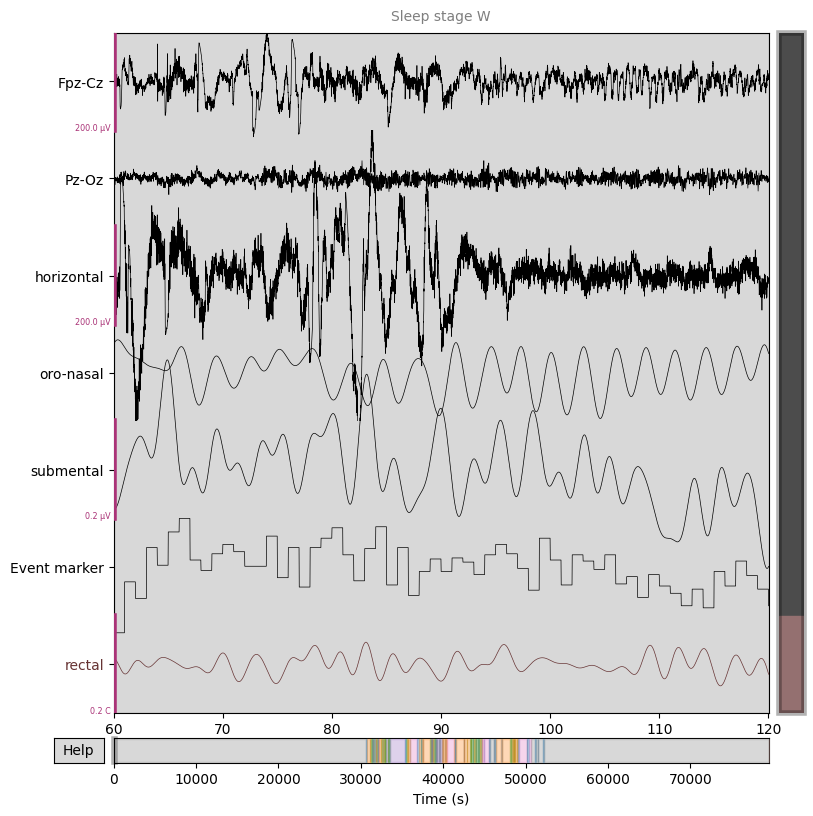
\includegraphics[width=\linewidth]{Sleep EDF Data Visulization.png} % Replace with your actual figure
			\caption{Sleep Stage Representation}
		\end{figure}
	\end{columns}
\end{frame}
   


 \begin{frame}{Proposed Architecture}
	\small
	\begin{columns}
		\begin{column}{0.6\textwidth}
			The proposed system processes EEG data through cleaning, normalization, and encoding before feeding it into neural models. It supports Dense, RNN, LSTM, and Bi-LSTM architectures with dropout layers for regularization. The models classify sleep stages (W, N1, N2, N3, REM) based on processed input features.
		\end{column}
		\begin{column}{0.3\textwidth}
			\centering
			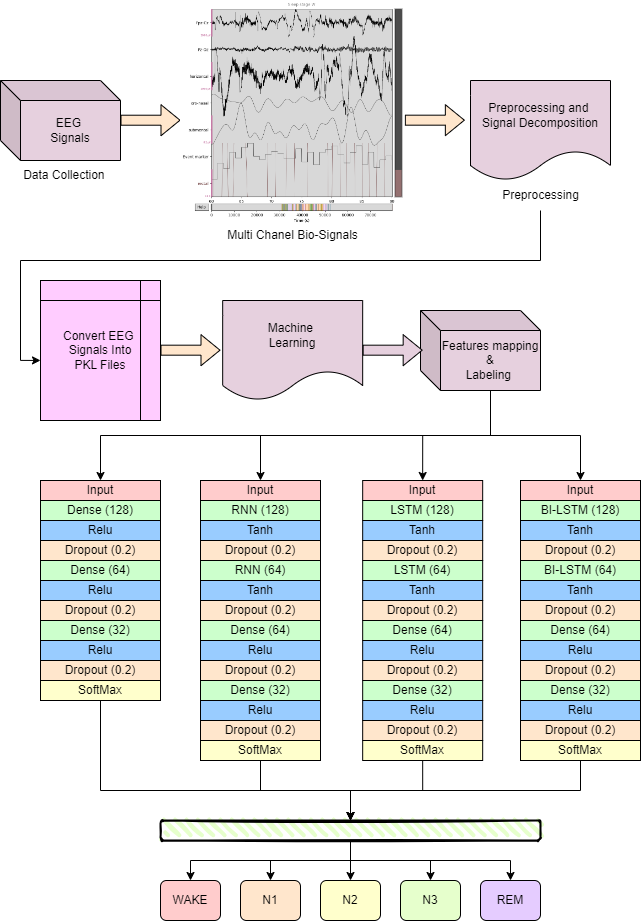
\includegraphics[width=\linewidth]{images/paper_2/aRCHITECHTURE 2} \\
			\textbf{Figure:} Proposed System Architecture
		\end{column}
	\end{columns}
\end{frame}



\begin{frame}{Methodology: Overview and Data Samples}
		\centering
	\small
	\textbf{Proposed System Architecture:} \\[5pt]

	\begin{tabular}{|c|p{0.63\textwidth}|}
		\hline
		\textbf{Component} & \textbf{Description} \\
		\hline
		Input & Sleep EEG Data (.pkl format) \\
		\hline
		Preprocessing & Normalization, Label Encoding, One-hot Encoding, Reshaping \\
		\hline
		Model & Neural Network (Dense / RNN / LSTM / Bi-LSTM) \\
		\hline
		Output & Predicted Sleep Stage (W, N1, N2, N3, REM) \\
		\hline
	\end{tabular} \\[10pt]
	
	\textbf{Sample Input Features and Labels:} \\[5pt]
	\centering
	\begin{tabular}{|p{0.63\textwidth}|c|}
		\hline
		\textbf{Input Features (x)} & \textbf{Label (y)} \\
		\hline
		{[0.059, 0.596, -0.193, ..., -0.601, 0.201]} & W \\
		\hline
		{[-0.022, -0.107, -0.135, ..., 0.038, 0.103]} & W \\
		\hline
		{[... (more samples)]} & N1 \\
		\hline
	\end{tabular} \\[5pt]
	
 
	
\end{frame}


 
 
 






\begin{frame}{Preprocessing Workflow}
	\textbf{Steps involved in data preparation:} \\[10pt]
	\begin{itemize}
		\item \textbf{Loading Data:} Sleep stage data is loaded from `.pkl` files in preprocessed directories.
		\item \textbf{Handling Test Sets:} Ensured test data availability by splitting the training set if necessary.
		\item \textbf{Normalization:} Standardized input features to have zero mean and unit variance.
		\item \textbf{Label Encoding:} Converted sleep stage labels into numerical format.
		\item \textbf{One-Hot Encoding:} Transformed numerical labels into one-hot vectors.
		\item \textbf{Reshaping:} Adjusted input dimensions for model compatibility.
	\end{itemize}
\end{frame}


 

 
 


\begin{frame}{Simple Neural Network Architecture}
	\centering
	\small
	\begin{tabular}{|c|c|c|}
		\hline
		\textbf{Layer Type} & \textbf{Neurons/Units} & \textbf{Activation Function} \\
		\hline
		Input Layer & X\_train & - \\
		\hline
		Dense Layer & 128 & ReLU \\
		\hline
		Dropout Layer & - & 0.2 \\
		\hline
		Dense Layer & 64 & ReLU \\
		\hline
		Dropout Layer & - & 0.2 \\
		\hline
		Dense Layer & 32 & ReLU \\
		\hline
		Dropout Layer & - & 0.2 \\
		\hline
		Output Layer & Number of Classes & Softmax \\
		\hline
	\end{tabular}
	
	\vspace{1em}
	\textit{Model:  Fully Dense Connected Neural Network}
\end{frame}


\begin{frame}{Simple RNN Architecture}
	\centering
	\small
	\begin{tabular}{|c|c|c|}
		\hline
		\textbf{Layer Type} & \textbf{Neurons/Units} & \textbf{Activation Function} \\
		\hline
		Input Layer & X\_train & - \\
		\hline
		RNN Layer 1 & 128 & Tanh \\
		\hline
		Dropout Layer & - & 0.2 \\
		\hline
		RNN Layer 2 & 64 & Tanh \\
		\hline
		Dropout Layer & - & 0.2 \\
		\hline
		Dense Layer & 64 & ReLU \\
		\hline
		Dropout Layer & - & 0.2 \\
		\hline
		Dense Layer & 32 & ReLU \\
		\hline
		Dropout Layer & - & 0.2 \\
		\hline
		Output Layer & Number of Classes & Softmax \\
		\hline
	\end{tabular}
	
	\vspace{1em}
	\textit{Model:  Recurrent Neural Network}
\end{frame}


\begin{frame}{LSTM Architecture}
	\centering
	\small
	\begin{tabular}{|c|c|c|}
		\hline
		\textbf{Layer Type} & \textbf{Neurons/Units} & \textbf{Activation Function} \\
		\hline
		Input Layer & X\_train & - \\
		\hline
		LSTM Layer 1 & 128 & Tanh \\
		\hline
		Dropout Layer & - & 0.2 \\
		\hline
		LSTM Layer 2 & 64 & Tanh \\
		\hline
		Dropout Layer & - & 0.2 \\
		\hline
		Dense Layer & 64 & ReLU \\
		\hline
		Dropout Layer & - & 0.2 \\
		\hline
		Dense Layer & 32 & ReLU \\
		\hline
		Dropout Layer & - & 0.2 \\
		\hline
		Output Layer & Number of Classes & Softmax \\
		\hline
	\end{tabular}
	
	\vspace{1em}
	\textit{Model: Long Short-Term Memory Network}
\end{frame}


\begin{frame}{Bidirectional LSTM Architecture}
	\centering
	\small
	\begin{tabular}{|c|c|c|}
		\hline
		\textbf{Layer Type} & \textbf{Neurons/Units} & \textbf{Activation Function} \\
		\hline
		Input Layer & X\_train & - \\
		\hline
		Bi-LSTM Layer 1 & 128 & Tanh \\
		\hline
		Dropout Layer & - & 0.2 \\
		\hline
		Bi-LSTM Layer 2 & 64 & Tanh \\
		\hline
		Dropout Layer & - & 0.2 \\
		\hline
		Dense Layer & 64 & ReLU \\
		\hline
		Dropout Layer & - & 0.2 \\
		\hline
		Dense Layer & 32 & ReLU \\
		\hline
		Dropout Layer & - & 0.2 \\
		\hline
		Output Layer & Number of Classes & Softmax \\
		\hline
	\end{tabular}
	
	\vspace{1em}
	\textit{Model: Bidirectional LSTM Network}
\end{frame}

\begin{frame}{Testing Data Distribution Analysis}

    \begin{columns}

        % Left Column: Explanation
        \column{0.50\textwidth}
        \textbf{Why Ensure Balanced Testing Data?}
        \begin{itemize}
     \item Prevents bias toward majority classes.
        \item Ensures the model's performance is fairly evaluated.
        \item Helps achieve reliable generalization across all sleep stages.
           \item The figure shows the normalized class distribution during testing.
        \item Each class maintains an equalized density, avoiding class imbalance.
        \item This confirms that the model's evaluation is not biased toward any specific sleep stage.
        \end{itemize}

        % Right Column: Sampling Density Plot
        \column{0.50\textwidth}
        \centering
        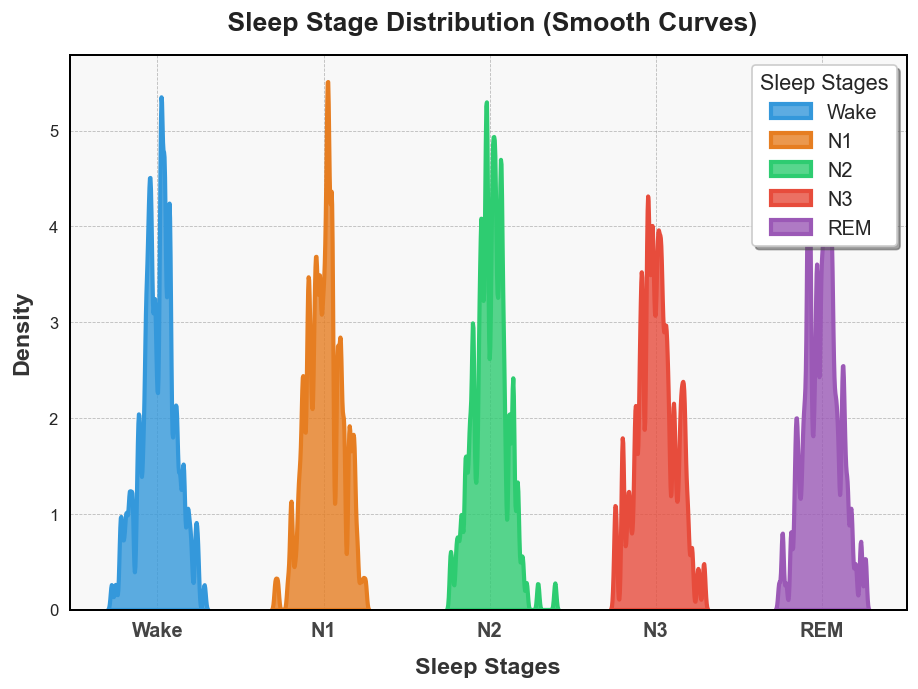
\includegraphics[width=0.9\linewidth]{figures/sample distribution plot pdf.png} % Replace with actual figure
        \vspace{5pt}
        {\textcolor{uwopurple}{\small Sampling Density Plot Showing Balanced Class Distribution}}

    \end{columns}

\end{frame}


\begin{frame}{Model Performance: Training vs Testing}

    \begin{columns}

        % Left Column: Accuracy Plot
        \column{0.50\textwidth}
        \centering
        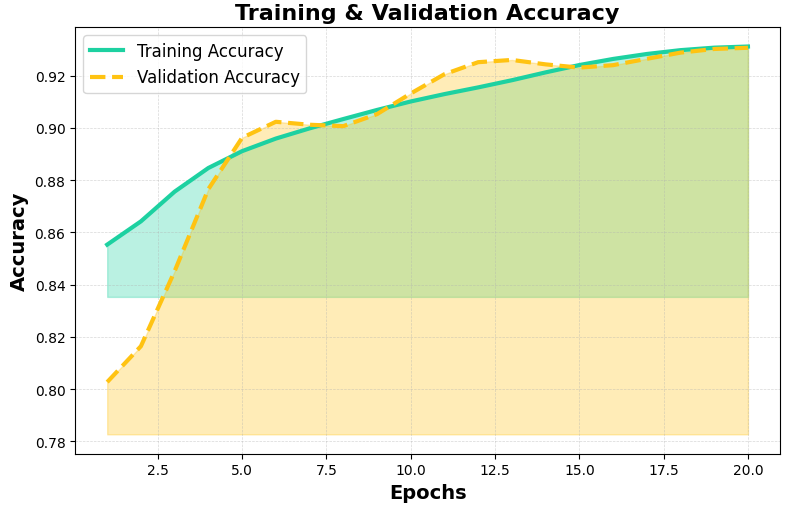
\includegraphics[width=1\linewidth]{figures/accuracy plot.png} % Replace with actual file
        \captionof{figure}{\textcolor{uwopurple}{ Accuracy Curve}}

        % Right Column: Loss Plot
        \column{0.50\textwidth}
        \centering
        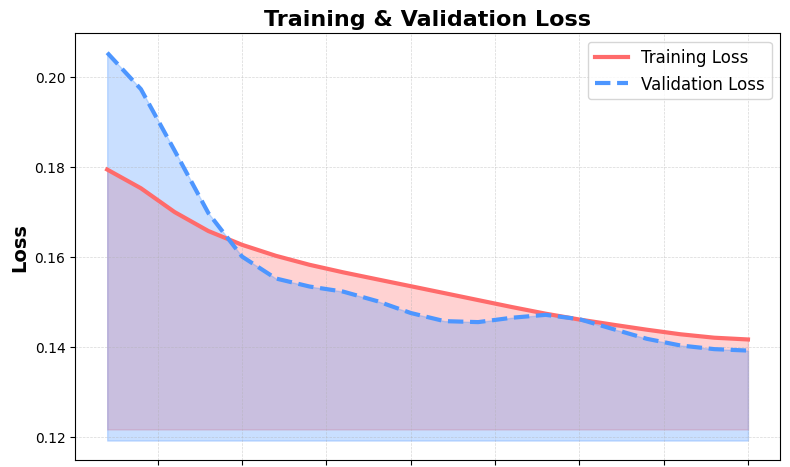
\includegraphics[width=1\linewidth]{figures/loss plot.png} % Replace with actual file
        \captionof{figure}{\textcolor{uwopurple}{ Loss Curve}}

    \end{columns}

\end{frame}



\begin{frame}{Model Evaluation: Confusion Matrix}

    \begin{columns}

        % Left Column: Precision, Recall, F1-Score Formulas
        \column{0.50\textwidth}
        \textbf{Performance Metrics}
        \vspace{10pt}
        
        \textbf{Precision:} 
        \[
        \text{Precision} = \frac{TP}{TP + FP}
        \]
        
        \textbf{Recall:} 
        \[
        \text{Recall} = \frac{TP}{TP + FN}
        \]

        \textbf{F1-Score:}
        \[
        \text{F1-Score} = \frac{2 \times \text{Precision} \times \text{Recall}}{\text{Precision} + \text{Recall}}
        \]

        \vspace{5pt}
        These metrics ensure a balanced evaluation of model performance across all classes.

        % Right Column: Confusion Matrix Plot
        \column{0.50\textwidth}
        \centering
        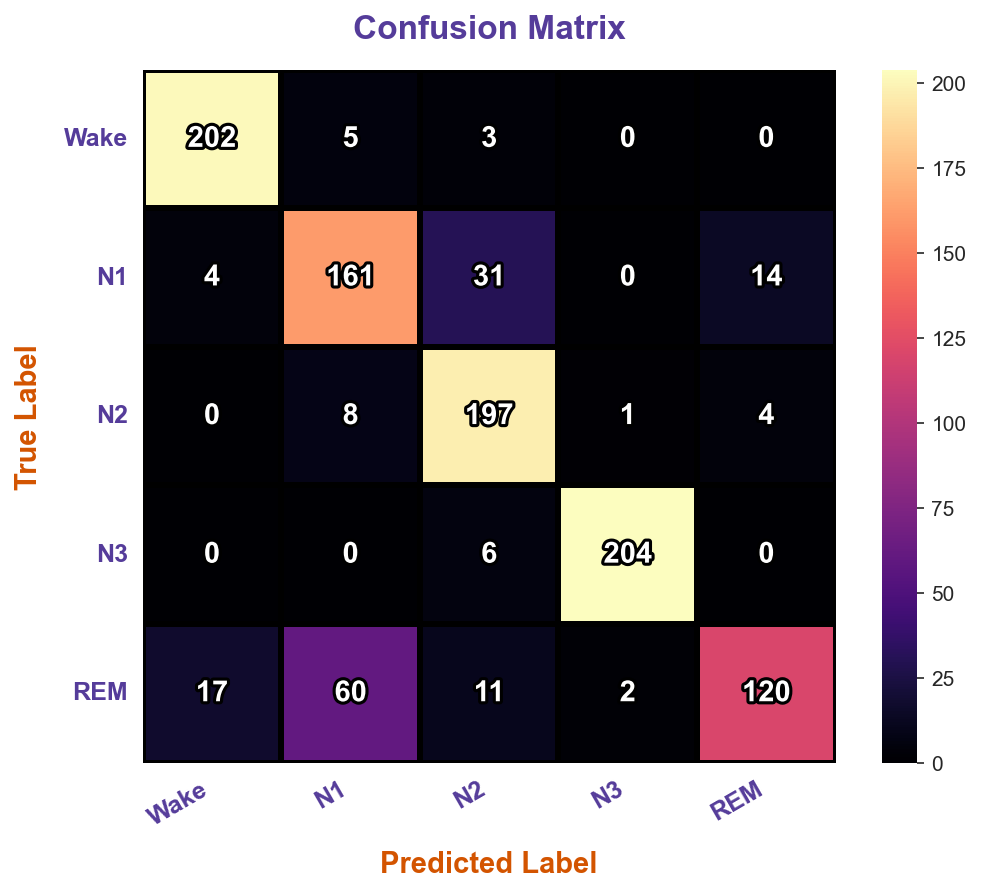
\includegraphics[width=0.9\linewidth]{figures/confusion matrix samples.png} % Replace with actual file
        \captionof{figure}{\textcolor{uwopurple}{Confusion Matrix }}

    \end{columns}

\end{frame}




\begin{frame}{Gradient Analysis: Training Progression}

    \begin{columns}

        % Left Column: Explanation of Training Behavior
        \column{0.50\textwidth}
        \textbf{Understanding Model Training Dynamics}
        \vspace{10pt}

      \begin{itemize}
            \item \textbf{Early Training (Epochs 0-5):} High loss, accuracy starts improving.
            \item \textbf{Mid Training (Epochs 5-15):} Loss steadily decreases, stable gradient flow.
            \item \textbf{Late Training (Epochs 15-20):} Accuracy plateaus, no severe overfitting.
        \end{itemize}

          \textbf{Conclusion:} The training process remains stable, with no vanishing or exploding gradients. 


        % Right Column: 3D Gradient Plot
        \column{0.50\textwidth}
        \centering
        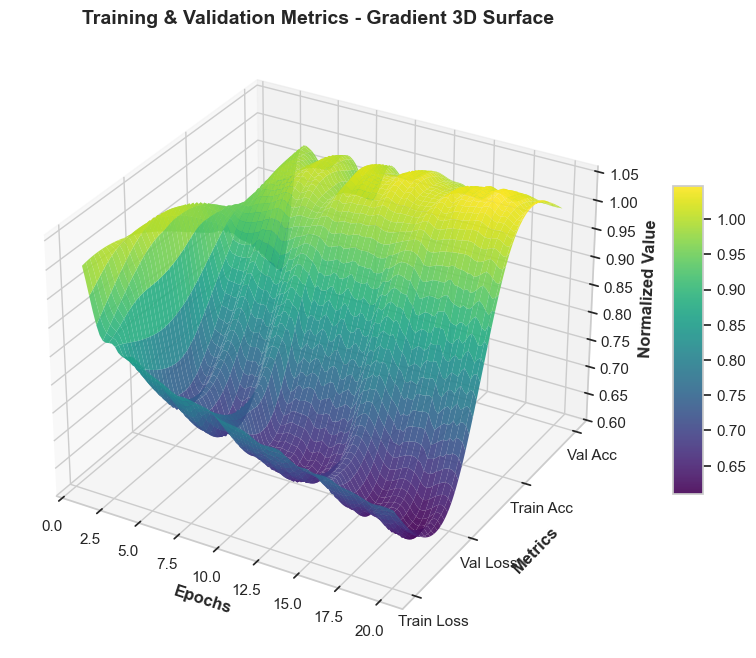
\includegraphics[width=0.9\linewidth]{figures/3d gradient.png} % Replace with actual file
        \captionof{figure}{\textcolor{purple}{Gradient 3D Surface: Training vs Validation Metrics}}

    \end{columns}

\end{frame}





\begin{frame}{Performance Metrics: Precision, Recall, F1-Score}

    \centering
    \textbf{Evaluating model performance across all classes using key metrics.}
    
    \vspace{10pt} % Add some space

    \begin{columns}
        % Left Column: Precision Bar Plot
        \column{0.33\textwidth}
        \centering
        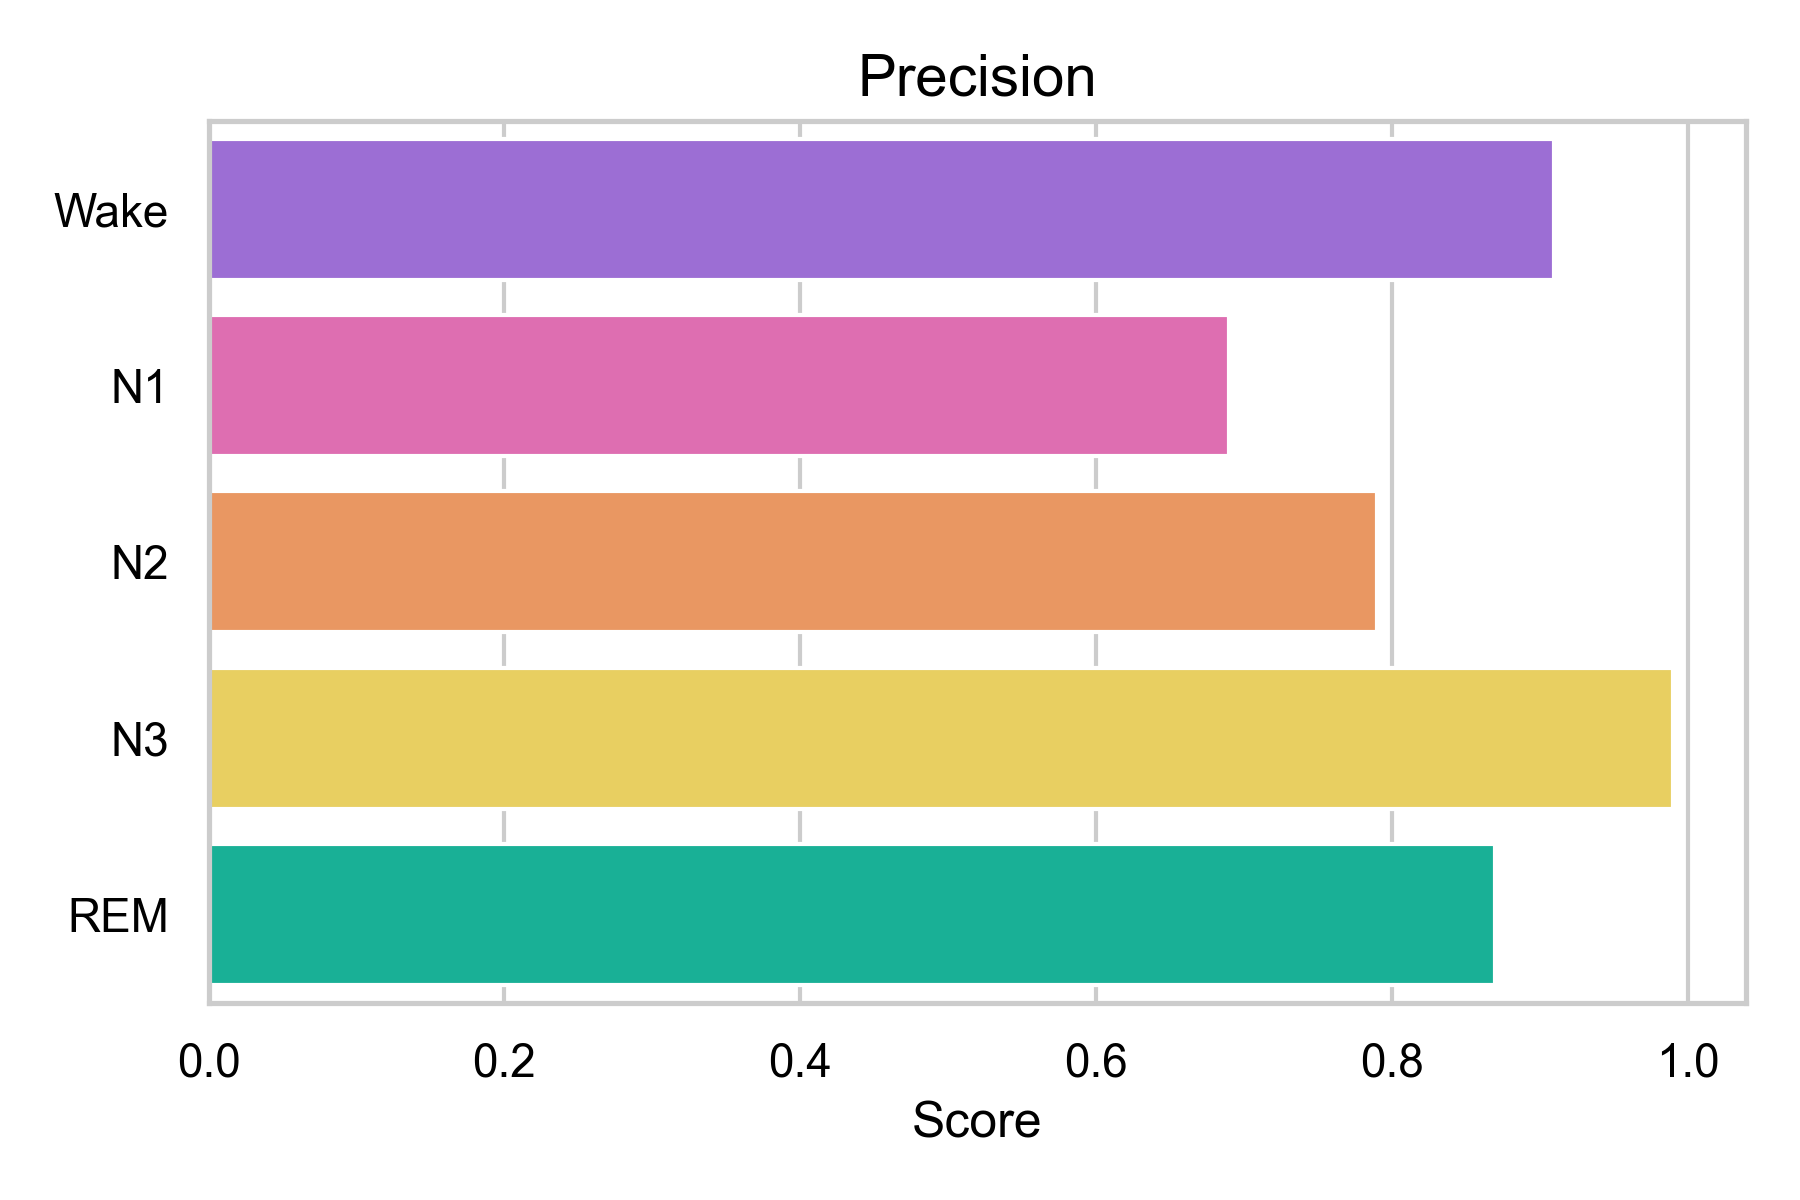
\includegraphics[width=\linewidth]{figures/precision_plot.png} % Replace with actual figure
        \captionof{figure}{\textcolor{purple}{Precision Scores per Class}}

        % Middle Column: Recall Bar Plot
        \column{0.33\textwidth}
        \centering
        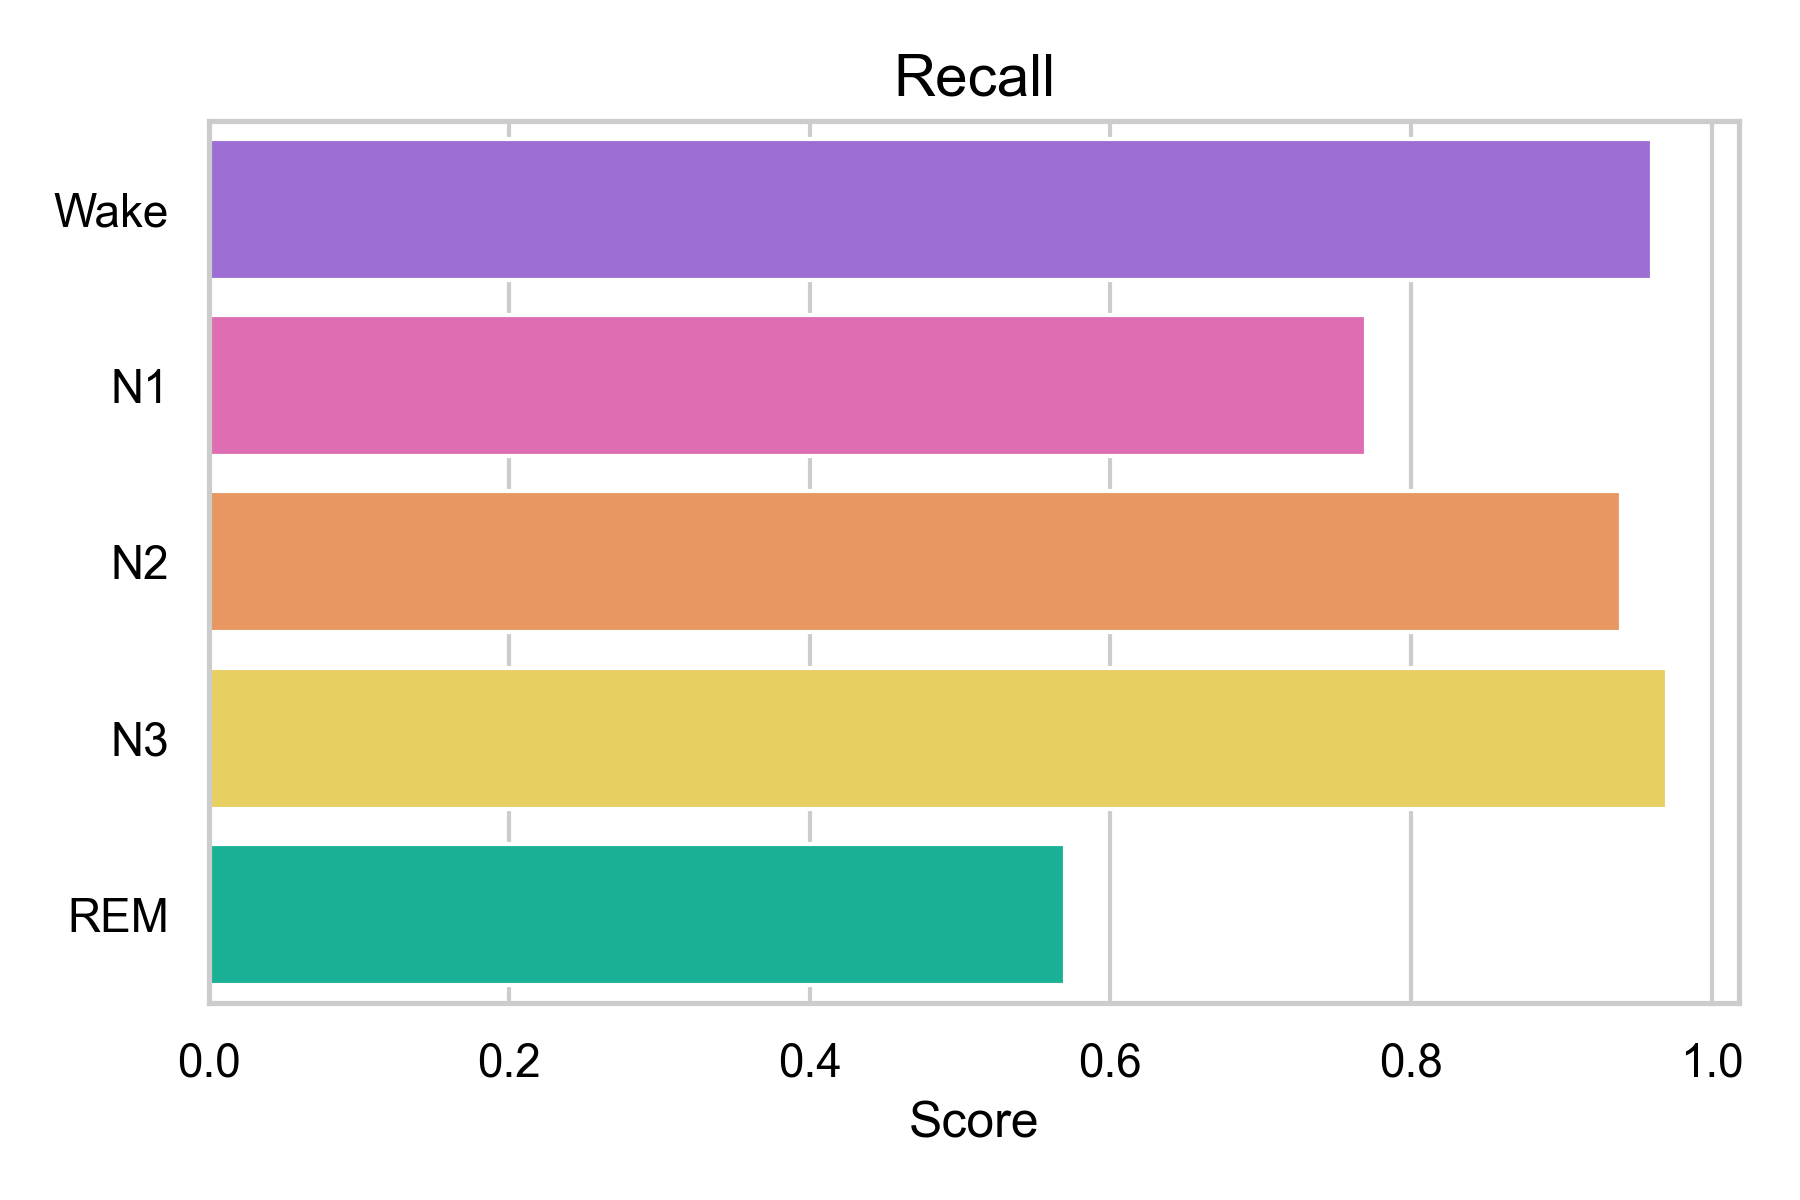
\includegraphics[width=\linewidth]{figures/recall_plot.png} % Replace with actual figure
        \captionof{figure}{\textcolor{purple}{Recall Scores per Class}}

        % Right Column: F1-Score Bar Plot
        \column{0.33\textwidth}
        \centering
        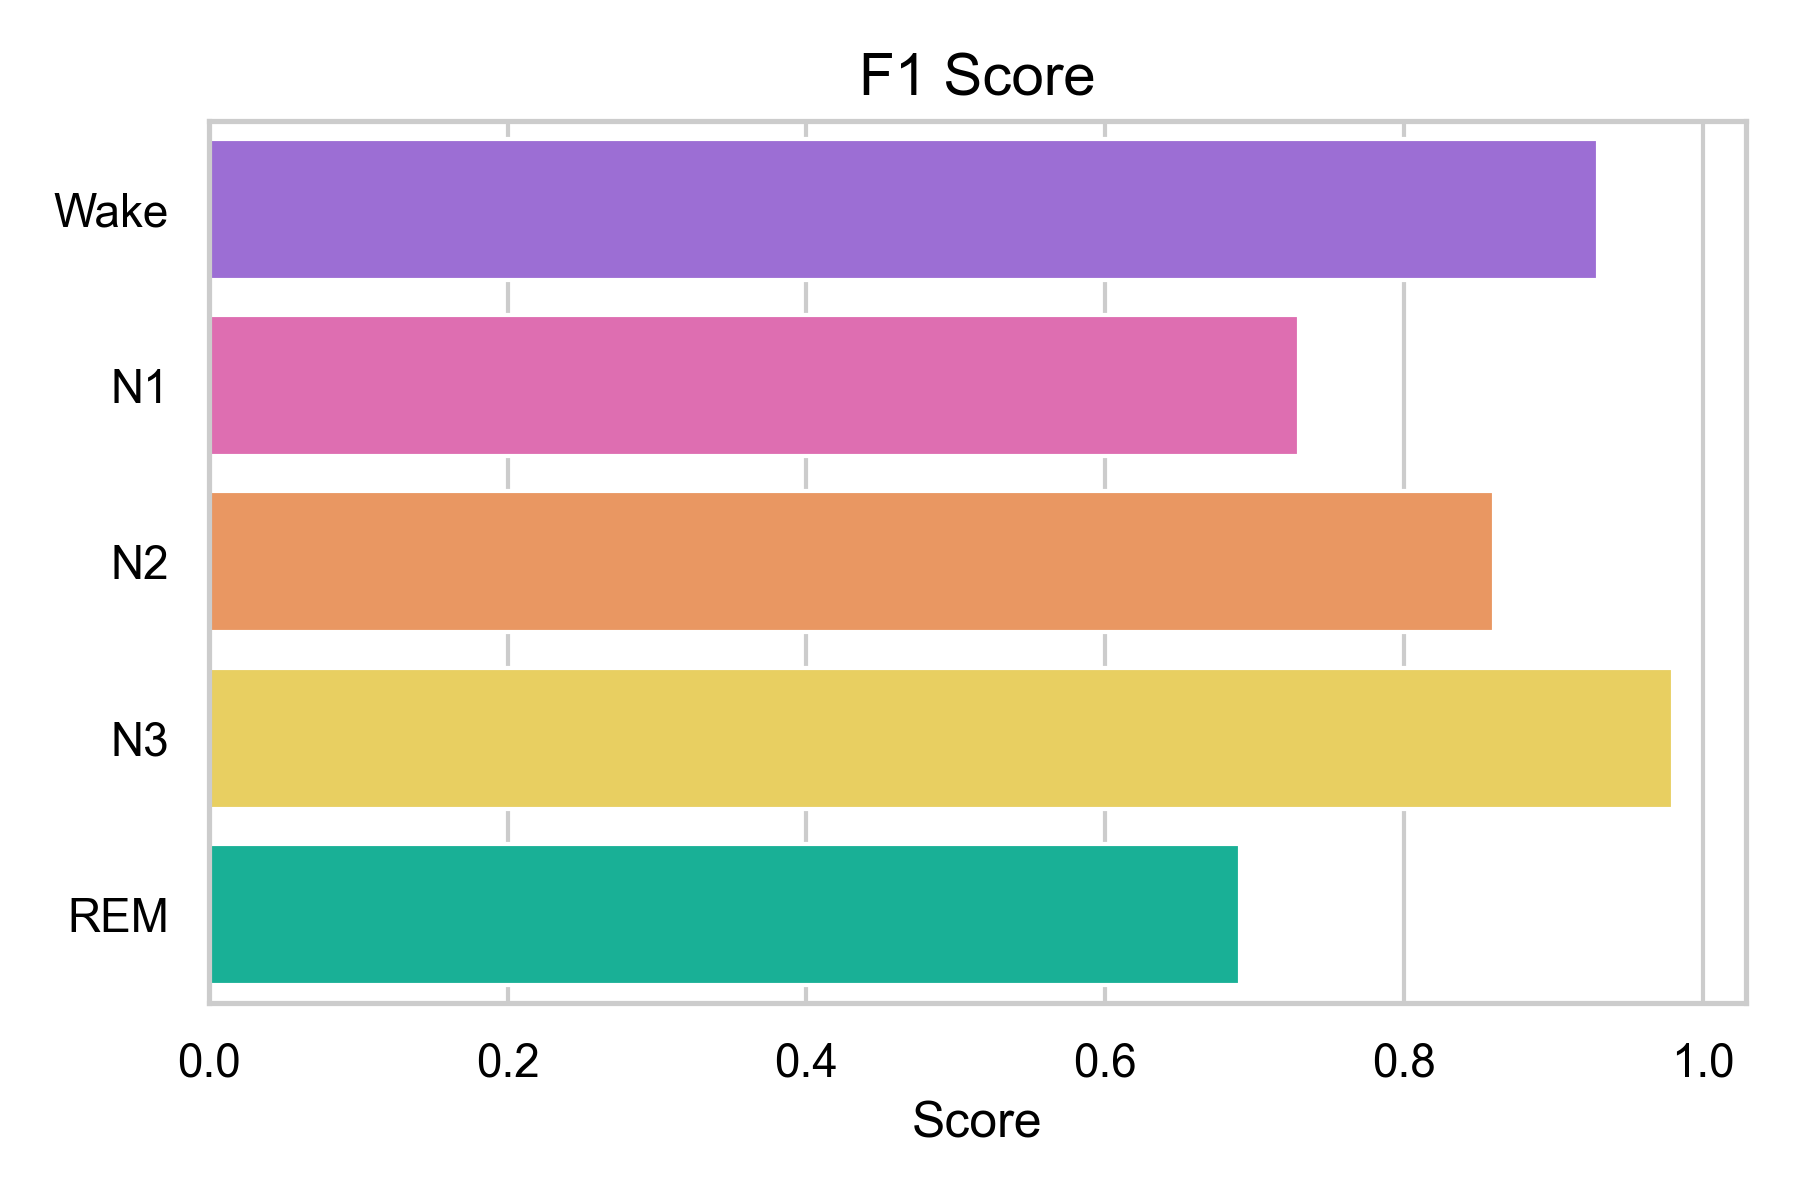
\includegraphics[width=\linewidth]{figures/f1_score_plot.png} % Replace with actual figure
        \captionof{figure}{\textcolor{purple}{F1 Scores per Class}}
    \end{columns}

\end{frame}

\begin{frame}{Feature Importance Analysis with LIME}

    \begin{columns}

        % Left Column: Explanation
        \column{0.5\textwidth}w
        \textbf{Understanding the contribution of different channels to model predictions.}

        \begin{itemize}
            \item We used \textbf{LIME} (Local Interpretable Model-agnostic Explanations) to analyze feature importance.
            \item The \textbf{EMG submental} and \textbf{EEG Pz-Oz} channels contribute the most to predictions.
            \item \textbf{EOG horizontal} has minimal importance, indicating lower relevance for classification.
            \item This insight helps optimize feature selection and improve model efficiency.
        \end{itemize}

        % Right Column: Figure
        \column{0.5\textwidth}
        \centering
        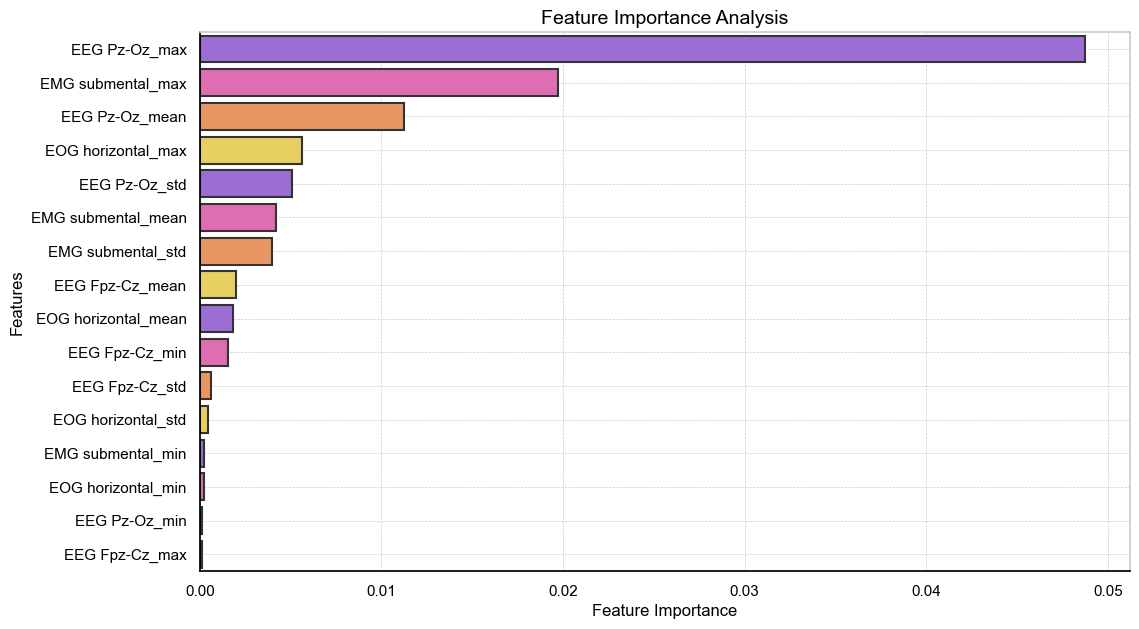
\includegraphics[width=0.9\linewidth]{figures/feature importance chanels analysis.png} % Replace with actual file path
        \captionof{figure}{\textcolor{purple}{Feature Importance Analysis for 4 Channels}}

    \end{columns}

\end{frame}




\begin{frame}{XAI: Enhancing Model Explainability}

    \textbf{Moving Towards Explainable AI for Sleep Staging}
    \vspace{0.5cm}
    
    \begin{itemize}
        \item \textbf{Why Explainability?}  
              - Medical experts need transparency in AI decisions for trust and adoption.  
              - Understanding how features influence sleep stage transitions is crucial.
              
        \item \textbf{Current Achievements:}  
              - \textcolor{blue}{\textbf{GCN:}} Captures spatial relationships between EEG channels.  
              - \textcolor{blue}{\textbf{Transformer:}} Captures temporal dependencies in sleep data.  
              - Achieved state-of-the-art accuracy using both approaches.
              
        \item \textbf{Next Steps:}  
              - Implement AI-driven methods to highlight critical sleep stage transition points.  
              - Develop feature attribution methods to understand the importance of each signal.  
              - Improve model interpretability to align with clinical expectations.
    \end{itemize}

\end{frame}



\begin{frame}{Future Plan: AI for Sleep Science and Clinical Use}

    \begin{columns}
        % Left Column: Explanation
        \column{0.55\textwidth}
        
        \textbf{Bridging AI and Healthcare}
        \begin{itemize}
            \item \textbf{Feature Importance:} Identify which EEG channels contribute most to predictions.
            \item \textbf{Clinical Relevance:} Provide insights that can be validated by sleep specialists.
            \item \textbf{Graph + Transformer Insights:}
            \begin{itemize}
                \item \textcolor{blue}{\textbf{GCN:}} Capturing inter-channel spatial dependencies.
                \item \textcolor{blue}{\textbf{Transformer:}} Learning sequential patterns across sleep cycles.
            \end{itemize}

                    \end{itemize}

        % Right Column: Block Diagram
       % Right Column: Block Diagram
\column{0.45\textwidth}
\centering
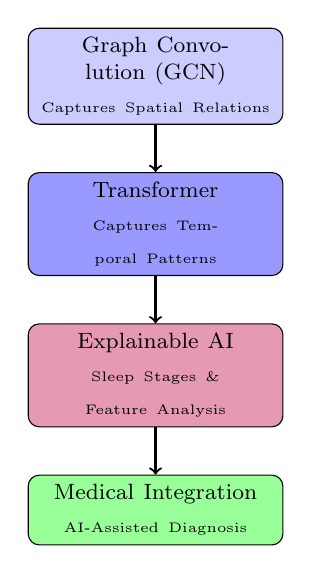
\begin{tikzpicture}
    % Nodes
    \node[draw, text width=3cm, align=center, fill=blue!20, rounded corners] 
        (gcn) {\footnotesize Graph Convolution (GCN) \\ \tiny Captures Spatial Relations};
        
    \node[draw, text width=3cm, align=center, fill=blue!40, rounded corners, below=0.6cm of gcn] 
        (transformer) {\footnotesize Transformer \\ \tiny Captures Temporal Patterns};
        
    \node[draw, text width=3cm, align=center, fill=purple!40, rounded corners, below=0.6cm of transformer] 
        (explainable) {\footnotesize Explainable AI \\ \tiny Sleep Stages \& Feature Analysis};
        
    \node[draw, text width=3cm, align=center, fill=green!40, rounded corners, below=0.6cm of explainable] 
        (medical) {\footnotesize Medical Integration \\ \tiny AI-Assisted Diagnosis};

    % Arrows
    \draw[->, thick] (gcn) -- (transformer);
    \draw[->, thick] (transformer) -- (explainable);
    \draw[->, thick] (explainable) -- (medical);
\end{tikzpicture}

    \end{columns}

\end{frame}

\begin{frame}{Conclusion}
	\begin{block}{}
		Our proposed SleepGCN-Transformer model achieves \textbf{93.12\% training accuracy} and \textbf{93.04\% validation accuracy}, demonstrating its effectiveness in sleep stage classification. The integration of \textbf{Graph Convolution Networks (GCN)} captures spatial dependencies across EEG, EOG, and EMG channels, while the \textbf{Transformer} extracts temporal patterns. The use of \textbf{Focal Loss} enhances class balancing, improving performance on underrepresented sleep stages. Feature importance analysis highlights \textbf{EMG and EEG Pz-Oz} as key predictors. This robust approach lays the foundation for future work in \textbf{Explainable AI}, enabling medical professionals to interpret AI-driven sleep diagnostics effectively.
	\end{block}
\end{frame}

\begin{frame}{Publications}
	\begin{block}{}
		\textbf{1. Automated Sleep Staging System with EEG Signal using Machine Learning Techniques} \\
		Santosh Kumar Satapathy, Tanmay Rathod, Nibedita Das, Rajesh Kumar Mohapatra, Suren Sahu, Jaynil Joshi, 2025 IEEE International Conference on Interdisciplinary Approaches in Technology and Management for Social Innovation (IATMSI). \url{https://ieeexplore.ieee.org/document/10985276} \\
		
		\textbf{2. Automated Sleep Staging System Using EEG Signal Feature-Based Classification by Machine Learning Techniques} \\
		Tanmay Rathod, Santosh Kumar Satapathy, Nibedita Das, Rajesh Kumar Mohapatra, Suren Kumar Sahu, Vaishvi R Shah, 2024 IEEE 8th International Conference on Information and Communication Technology (CICT). \url{https://ieeexplore.ieee.org/document/10899578}
		
		\textbf{3. SleepGCN-Transformer: A Hybrid Graph-Convolutional Approach for EEG-based Sleep Staging} \\
		Tanmay Rathod et al., submitted to \textit{Biomedical Signal Processing and Control}, May 2025 (under review).
		
		\end{block}
\end{frame}

\begin{frame}{Thank You !}
	\begin{block}{}
		For inquiries or collaboration, contact the author via the following: \\
		
		\textbf{Email:} \href{mailto:tanmayrathod777@gmail.com}{tanmayrathod777@gmail.com} \\
		\textbf{Phone:} +91 90165 89777 \\
		\textbf{GitHub:} \url{https://github.com/tanmay007thor} \\
		\textbf{IEEE Xplore:} \url{https://ieeexplore.ieee.org/author/577823064896395} \\
		\textbf{Portfolio:} \url{https://tanmay-dev.netlify.app/} \\
		\textbf{LinkedIn:} \url{https://www.linkedin.com/in/tanmay-rathod-15a332230}
	\end{block}
\end{frame}


\end{document}